% =================================================================================================
% File:			dettaglio_delle_verifiche_tramite_analisi.tex
% Description:	Definisce le verifiche effettuate tramite analisi
% Created:		2014/03/05
% Author:		Faccin Nicola
% Email:		faccin.nicola@mashup-unipd.it
% =================================================================================================
% Modification History:
% Version		Modifier Date		Change											Author
% 0.0.1 		2014/01/11 			iniziata stesura appendice					Lorenzo C.
% =================================================================================================
%% Version		Modifier Date		Change											Author
% 1.0.1 		2015/03/17 			iniziata stesura appendice B				Nicola F.
% =================================================================================================
%


% CONTENUTO DEL CAPITOLO

\section{Dettaglio delle verifiche tramite analisi}
	\subsection{Ricerca ed implementazione degli strumenti}
		\subsubsection{Processi}
		Il seguente grafico deriva dall'analisi dei ticket pianificati, svolti, approvati e verificati dal gruppo in relazione alle date in cui hanno cambiato stato. \\ \\
		Come si può notare in figura 3, c'è una rapida crescita di task pianificati nelle date dei verbali interni che corrispondono alle riunioni del gruppo, nonché ai verbali interni. Verso la fine della fase si osserva un aumento dei task approvati e verificati, questo per tentare di completare tutti quelli pianificati entro la data di fine fase. Si nota in oltre che non tutti i task sono stati completati entro la fine della fase, questo andrà ad appesantire dunque la fase successiva che si verrà a trovare i task della fase precedente da completare.
			\begin{figure}[htbp]
				\centering
				\centerline{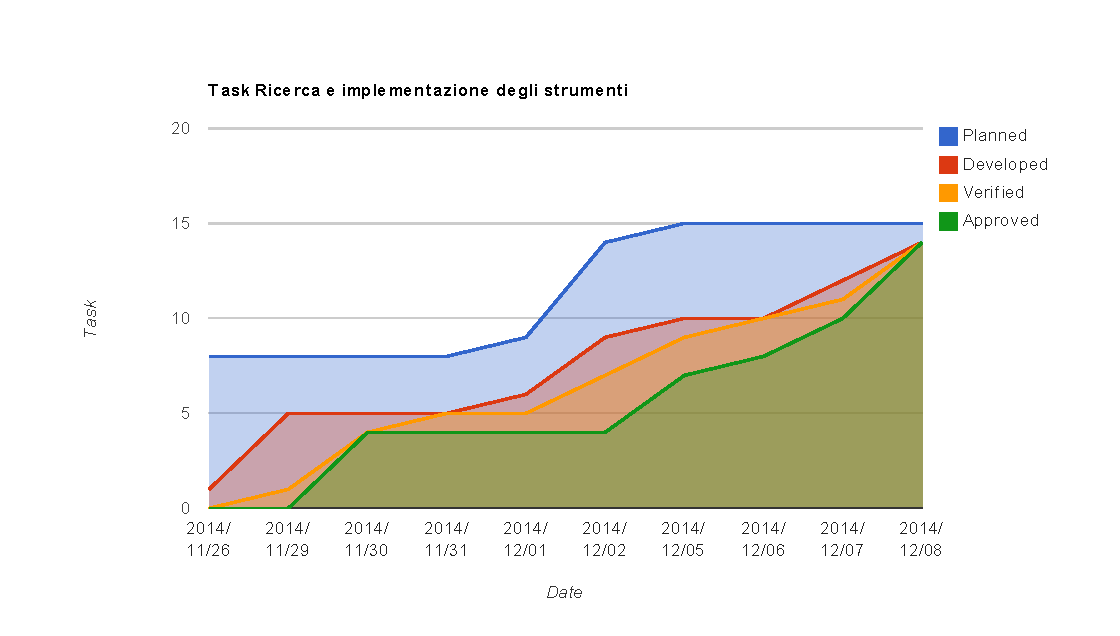
\includegraphics[scale=1]{images/Grafico_fase_1.pdf}}
				\caption{Grafico task Ricerca ed implementazione degli strumenti}
				\label{fig:taskfase1}
			\end{figure}
		\subsubsection{Documenti}
		Essendo in questa fase non presente ancora alcun documento, non è stato possibile verificarli e quindi avere dei valori da esporre. Per correttezza è stato comunque inserito il nome della fase.
	
	\subsection{Analisi dei requisiti}
		\subsubsection{Processi}
		La figura 4 rappresenta l'andamento dei task relativi a questa fase, si nota che dato l'inesperienza del gruppo e il tipo di fase in cui ci troviamo, inizialmente non ci sono molti task pianificati come ci si potrebbe aspettare in altre fasi. Il gruppo ha proseguito a pianificare pochi task alla volta fino al primo incontro con il proponente, dal 2015/01/14 si osserva infatti un notevole picco inizialmente per i Planned ma poi anche per i Developed Verified e Approved. 
			\begin{figure}[htbp]
				\centering
				\centerline{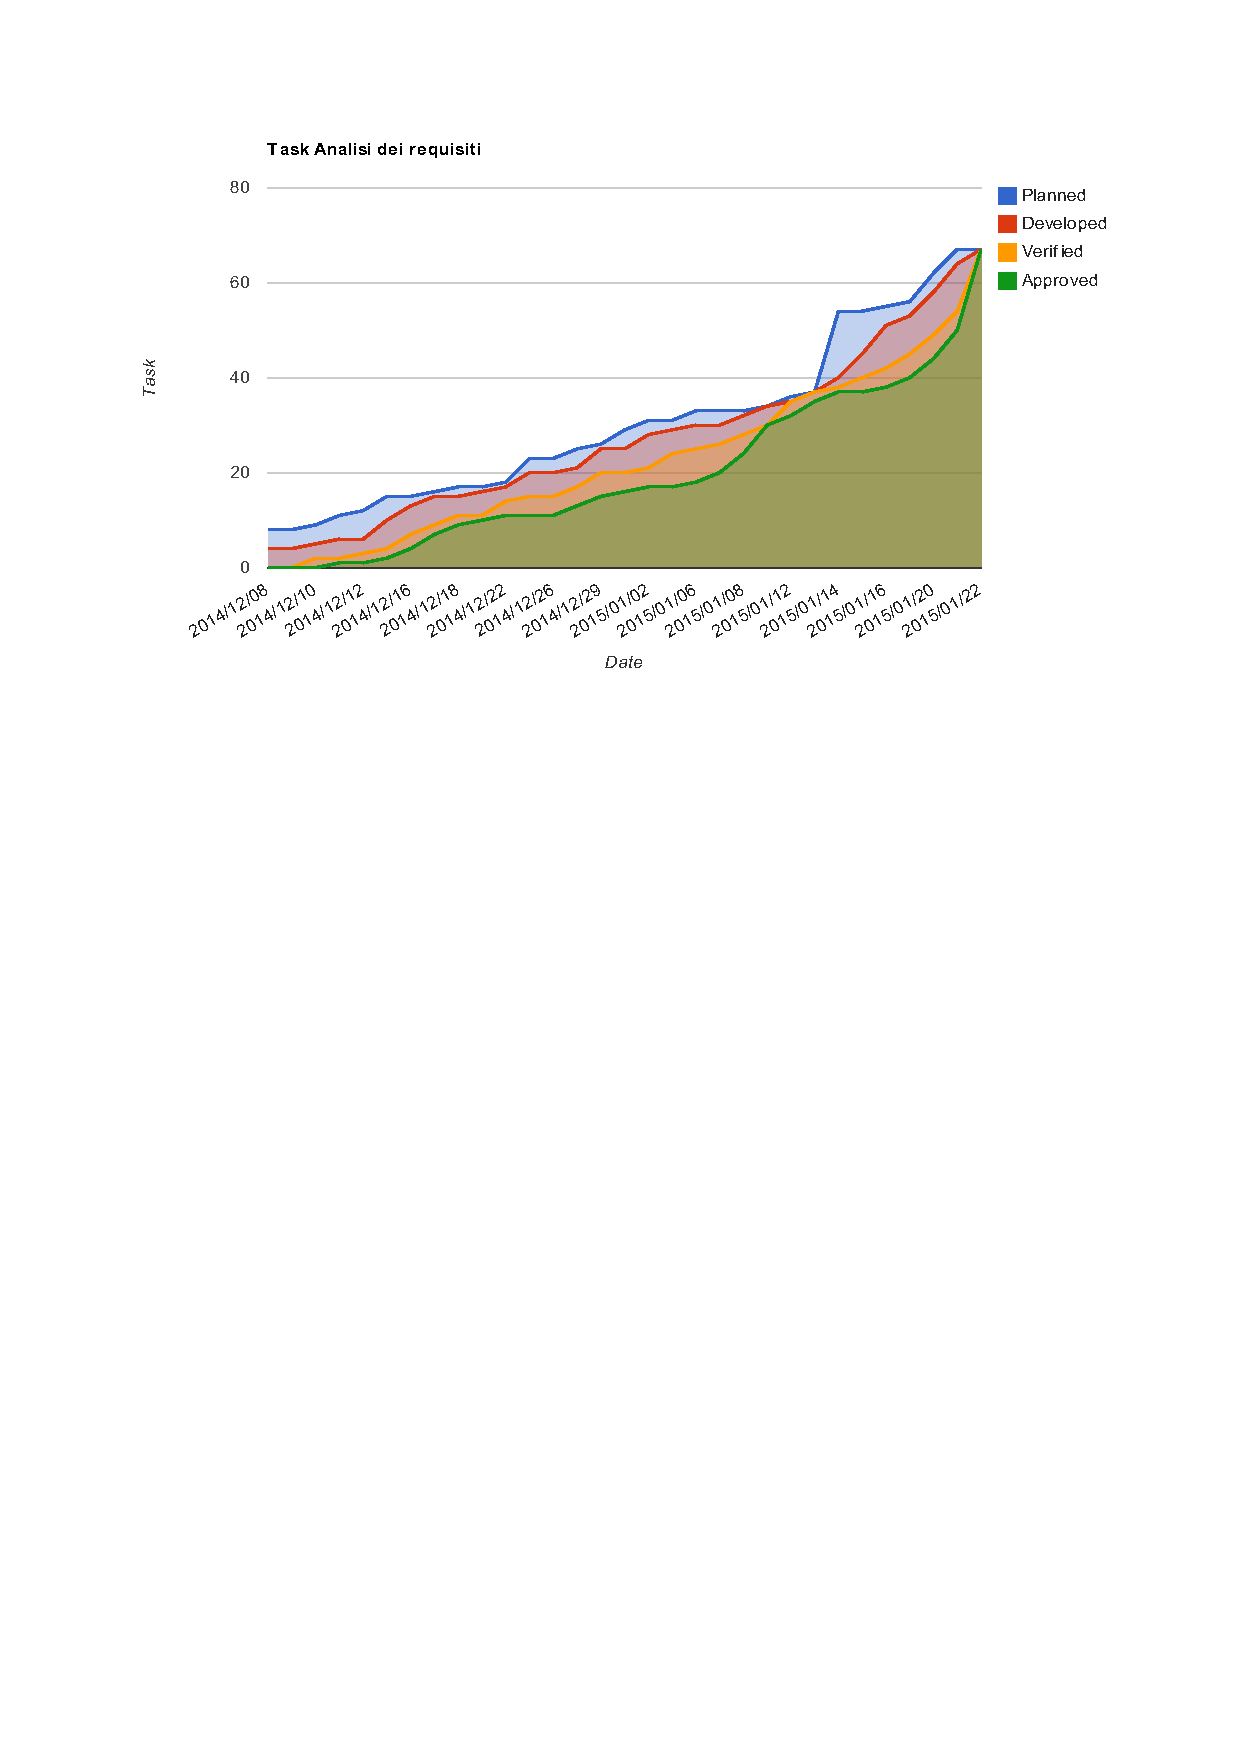
\includegraphics[scale=1]{images/Grafico_fase_2.pdf}}
				\caption{Grafico task Analisi dei requisiti}
				\label{fig:taskfase2}
			\end{figure}
	 	\subsubsection{Documenti}
		\begin{table}[!ht]
			\begin{center}
				\begin{tabularx}{0.9\textwidth}{|l|l|X|}
					\hline
					\textbf{Nome documento} & \textbf{Valore indice} & \textbf{Esito}\\
					\hline						
					\docNameVersionAdR & 56 & \textcolor{green}{Superato}\\
					\hline
					\docNameVersionGlo & 50 & \textcolor{green}{Superato}\\
					\hline					
					\docNameVersionNdP & 54 & \textcolor{green}{Superato}\\
					\hline					
					\docNameVersionPdP & 55 & \textcolor{green}{Superato}\\
					\hline					
					\docNameVersionPdQ & 55 & \textcolor{green}{Superato}\\
					\hline					
					\docNameVersionSdF & 48 & \textcolor{green}{Superato}\\
					\hline				
				\end{tabularx}
			\end{center}
			\caption{Risultati indice Gulpease}
		\end{table}
		\subsection{Analisi di dettaglio}
		\subsubsection{Processi}
		Vengono qui riportati i valori degli indici di budget e schedule variance per le attività della fase \textbf{Analisi di dettaglio}.
			\begin{table}[!ht]
			\begin{center}
				\begin{tabularx}{0.9\textwidth}{|l|l|X|}
					\hline
					\textbf{Attività} & \textbf{Schedule variance} & \textbf{Budget variance}\\
					\hline						
					\docNameVersionAdR & ?? & ??\\
					\hline
					\docNameVersionGlo & ?? & ??\\
					\hline					
					\docNameVersionNdP & ?? & ??\\
					\hline					
					\docNameVersionPdP & ?? & ??\\
					\hline					
					\docNameVersionPdQ & ?? & ??\\
					\hline					
					\docNameVersionSdF & ?? & ??\\
					\hline				
				\end{tabularx}
			\end{center}
		\caption{Esiti verifica sui processi fase - Analisi di dettaglio}
	\end{table}
	Complessivamente si registrano:
	\begin{itemize}
	\item \textbf{Schedule variance:} ;
	\item \textbf{Budget variance:} .
	\end{itemize}
	 	\subsubsection{Documenti}
		\begin{table}[!ht]
			\begin{center}
				\begin{tabularx}{0.9\textwidth}{|l|l|X|}
					\hline
					\textbf{Nome documento} & \textbf{Valore indice} & \textbf{Esito}\\
					\hline						
					\docNameVersionAdR & ?? & \textcolor{green}{Superato}\\
					\hline
					\docNameVersionGlo & ?? & \textcolor{green}{Superato}\\
					\hline					
					\docNameVersionNdP & ?? & \textcolor{green}{Superato}\\
					\hline					
					\docNameVersionPdP & ?? & \textcolor{green}{Superato}\\
					\hline					
					\docNameVersionPdQ & ?? & \textcolor{green}{Superato}\\
					\hline					
					\docNameVersionSdF & ?? & \textcolor{green}{Superato}\\
					\hline				
				\end{tabularx}
			\end{center}
			\caption{Risultati indice Gulpease}
		\end{table}
		\subsection{Progettazione architetturale}
		\subsubsection{Processi}
		Vengono qui riportati i valori degli indici di budget e schedule variance per le attività della fase \textbf{Progettazione architetturale}.
			\begin{table}[!ht]
			\begin{center}
				\begin{tabularx}{0.9\textwidth}{|l|l|X|}
					\hline
					\textbf{Attività} & \textbf{Schedule variance} & \textbf{Budget variance}\\
					\hline						
					\docNameVersionAdR & ?? & ??\\
					\hline
					\docNameVersionGlo & ?? & ??\\
					\hline					
					\docNameVersionNdP & ?? & ??\\
					\hline					
					\docNameVersionPdP & ?? & ??\\
					\hline					
					\docNameVersionPdQ & ?? & ??\\
					\hline					
					\docNameVersionSdF & ?? & ??\\
					\hline		
					\docNameVersionST & ?? & ??\\
					\hline		
				\end{tabularx}
			\end{center}
		\caption{Esiti verifica sui processi fase - Progettazione architetturale}
	\end{table}
	Complessivamente si registrano:
	\begin{itemize}
	\item \textbf{Schedule variance:} ;
	\item \textbf{Budget variance:} .
	\end{itemize}
	 	\subsubsection{Documenti}
		\begin{table}[!ht]
			\begin{center}
				\begin{tabularx}{0.9\textwidth}{|l|l|X|}
					\hline
					\textbf{Nome documento} & \textbf{Valore indice} & \textbf{Esito}\\
					\hline						
					\docNameVersionAdR & ?? & \textcolor{green}{Superato}\\
					\hline
					\docNameVersionGlo & ?? & \textcolor{green}{Superato}\\
					\hline					
					\docNameVersionNdP & ?? & \textcolor{green}{Superato}\\
					\hline					
					\docNameVersionPdP & ?? & \textcolor{green}{Superato}\\
					\hline					
					\docNameVersionPdQ & ?? & \textcolor{green}{Superato}\\
					\hline					
					\docNameVersionSdF & ?? & \textcolor{green}{Superato}\\
					\hline	
					\docNameVersionST & ?? & \textcolor{green}{Superato}\\
					\hline			
				\end{tabularx}
			\end{center}
			\caption{Risultati indice Gulpease}
		\end{table}
		\subsection{Progettazione di dettaglio e codifica dei requisiti obbligatori}
		\subsubsection{Processi}
		Vengono qui riportati i valori degli indici di budget e schedule variance per le attività della fase \textbf{Progettazione di dettaglio e codifica dei requisiti obbligatori}.
			\begin{table}[!ht]
			\begin{center}
				\begin{tabularx}{0.9\textwidth}{|l|l|X|}
					\hline
					\textbf{Attività} & \textbf{Schedule variance} & \textbf{Budget variance}\\
					\hline						
					\docNameVersionAdR & ?? & ??\\
					\hline
					\docNameVersionGlo & ?? & ??\\
					\hline					
					\docNameVersionNdP & ?? & ??\\
					\hline					
					\docNameVersionPdP & ?? & ??\\
					\hline					
					\docNameVersionPdQ & ?? & ??\\
					\hline					
					\docNameVersionSdF & ?? & ??\\
					\hline				
				\end{tabularx}
			\end{center}
		\caption{Esiti verifica sui processi fase - Progettazione di dettaglio e codifica dei requisiti obbligatori}
	\end{table}
	Complessivamente si registrano:
	\begin{itemize}
	\item \textbf{Schedule variance:} ;
	\item \textbf{Budget variance:} .
	\end{itemize}
	 	\subsubsection{Documenti}
		\begin{table}[!ht]
			\begin{center}
				\begin{tabularx}{0.9\textwidth}{|l|l|X|}
					\hline
					\textbf{Nome documento} & \textbf{Valore indice} & \textbf{Esito}\\
					\hline						
					\docNameVersionAdR & ?? & \textcolor{green}{Superato}\\
					\hline
					\docNameVersionGlo & ?? & \textcolor{green}{Superato}\\
					\hline					
					\docNameVersionNdP & ?? & \textcolor{green}{Superato}\\
					\hline					
					\docNameVersionPdP & ?? & \textcolor{green}{Superato}\\
					\hline					
					\docNameVersionPdQ & ?? & \textcolor{green}{Superato}\\
					\hline					
					\docNameVersionSdF & ?? & \textcolor{green}{Superato}\\
					\hline				
				\end{tabularx}
			\end{center}
			\caption{Risultati indice Gulpease}
		\end{table}
	
\pagebreak